\documentclass[10pt]{beamer}

%%%
% PREAMBLE FOR THIS DOC 
%%%
%https://tex.stackexchange.com/questions/68821/is-it-possible-to-create-a-latex-preamble-header
\usepackage{/Users/miw267/Repos/latex_preamble/beamer_preamble}



%%% TRY TO RESHOW TOC AT EACH SECTION START (with current section highlighted)
% Reference: https://tex.stackexchange.com/questions/280436/how-to-highlight-a-specific-section-in-beamer-toc
\newcommand\tocforsect[2]{%
  \begingroup
  \edef\safesection{\thesection}
  \setcounter{section}{#1}
  \tableofcontents[#2,currentsection]
  \setcounter{section}{\safesection}
  \endgroup
}


%%%% HERES HOW TO DO IT CORRECTLY
% FIRST IN .STY FILE, DO
%\usetheme[sectionpage=none]{metropolis}
% THEN AT EACH SECTION DO
%\begin{frame}{Outline}
%  \tableofcontents[currentsection]	
%\end{frame}



%\setbeamertemplate{navigation symbols}{}
%\setbeamertemplate{footline}[frame number]{}

%%% THIS DOC ONLY
\usetikzlibrary{calc}


%%%
% DOCUMENT
%%%

\begin{document}

%\maketitle

%% Title page frame
%\begin{frame}
%    \titlepage 
%\end{frame}





\title{09/16/2026: Sets}
\author{CSCI 246: Discrete Structures}
\date{Textbook reference: Sec. 10, Scheinerman}

\begin{frame}
    \titlepage 
\end{frame}


\begin{frame}
\small 
\begin{mygreenbox}[title=Graded Quiz Pickup]
Quizzes are in the front of the room, grouped into four bins (A-G, H-L, M-R, S-Z) by last name. The quizzes are upside down with your last name on the back. Come find yours before, during, or after class.  Only turn the quiz over if it's yours.
\end{mygreenbox} 
\vfill 
\begin{myredbox}[title=Early Feedback]
\begin{enumerate}
	\item What do like about class so far / what's helping with your learning?
	\item What do dislike about class so far / what's interfering with your learning?
	\item Any other comments?
\end{enumerate}
\end{myredbox}
\vfill 

\begin{myyellowbox}[title=Today's Agenda]
\begin{itemize}
	\item Review group exercises  ($\approx$ 15 mins)
	\item Mini-lecture ($\approx$ 15 mins)
	\item Group exercises ($\approx$ 15 mins)
\end{itemize}

\end{myyellowbox}
\vfill 
\end{frame}



\begin{frame}{Study Guide For Quiz 3}

\footnotesize 
\begin{myredbox}[title=Readings]
Sec. 7 (Boolean Algebra)
\begin{itemize}
\item Know how to prove Props 7.1 and 7.3 using truth tables.
\item Understand the Boolean algebra properties listed in Theorem 7.2.  (What are they saying? Could you use them?)
\end{itemize}
Sec. 8 (Lists)
\begin{itemize}
\item Know how to solve examples 8.1, 8.3, 8.4, and 8.5
\item Know how to apply Theorems 8.2 and 8.6. 
\end{itemize}
Sec. 9 (Factorial)
\begin{itemize}
\item Know how to apply the definition of factorial.
\item Know how to justify why $0!=1$.
\item Understand how to read product notation.
\end{itemize}

\end{myredbox}

\vfill 

\begin{myyellowbox}[title=Group exercises]
Know how to do all of the group exercises from those course meetings.
\end{myyellowbox}

\end{frame}

\begin{frame}[standout]
Review group exercises
\end{frame}



\begin{frame}[standout]
Some notes on Sets I (Introduction, Subsets) 
\end{frame}


\begin{frame}{Subtopics from reading}
Scheinerman Sec. 10 (Sets I: Introduction, Subsets) covers the following subtopics
\begin{enumerate}
	\item Introduction to sets and set notation,
	\item How to show one set is a subset of the other,
	\item How to show two sets are equal, and
	\item How to count the number of subsets of a set.
\end{enumerate}

\vfill
Today's mini-lecture and group exercises focus on these subtopics. 
\end{frame}

%%%% Section
\begin{frame}[standout]
Outline for Mini-Lecture:
\begin{itemize}
\item \alert{\textbullet \quad Introduction to sets and set notation}
\item \textbullet \quad How to show two sets are equal
\item \textbullet \quad How to count the number of subsets
\end{itemize}
\end{frame}


\begin{frame}{Sets vs. lists}

\colorbox{yellow!30}{\textbf{Question:}} Where did Mike go on vacation last summer?

\vfill 
\pause 

\colorbox{green!30}{\textbf{Answer via list:}} Lists are \alert{ordered}.  I could perhaps answer in the order of the places I visited

\begin{center}
(Florida, camping in WA, Flathead Lake)	
\end{center}

\vfill
\pause 
Note that 

\begin{center}
\phantom{$\neq$} (Florida, camping, lake) $\neq$ (Florida, lake, camping) \\
 $\neq$ (camping, Florida, lake) $\neq$ (camping, lake, Florida) \\
  $\neq$ (lake, camping, Florida) $\neq$ (lake, Florida, camping) \\
\end{center}

\vfill 
\pause 
\colorbox{green!30}{\textbf{Answer via set:}} Sets are \alert{unordered}.   I could equivalently provide any of the following as a solution.

\begin{center}
\phantom{=} \{Florida, camping, lake\} =  \{Florida, lake, camping\} \\
 =  \{camping, Florida, lake\} = \{camping, lake, Florida\} \\
= \{lake, camping, Florida\} = \{lake, Florida, camping\} \\
\end{center}

	
\end{frame}


\begin{frame}{Three special sets of numbers}
\small 
\begin{mygreenbox}[title=Definition]
The \textbf{integers} are the positive whole numbers, the negative whole numbers, and zero.  That is, the set of integers, denoted by $\mathbb{Z}$ is
\[\mathbb{Z} = \set{\hdots, -3, -2, -1, 0, 1, 2, 3 \hdots}.\] 
\end{mygreenbox}
\vfill 
\pause 
\begin{mygreenbox}[title=Definition]
The \textbf{natural numbers} (denoted $\mathbb{N}$) are the non-negative integers; that is
\[\mathbb{N} = \set{0, 1, 2, 3 \hdots}.\] 
\end{mygreenbox}
\vfill 
\pause 

% --- Rational box with inline TikZ and an annotation that appears after a pause ---
\begin{mygreenbox}[title=Definition]
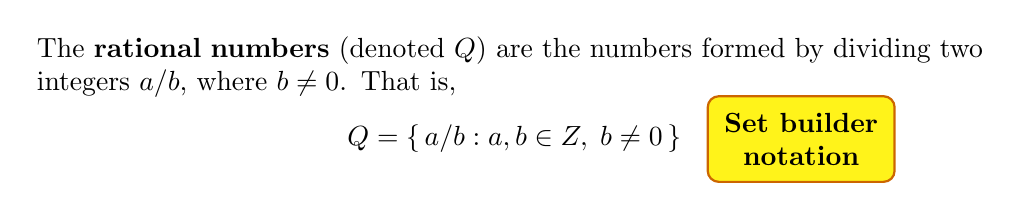
\begin{tikzpicture}[remember picture]
  % left text block (use most of the box width)
  \node[anchor=north,align=left,text width=\linewidth] (L) at (0,0) {%
    The \textbf{rational numbers} (denoted \(\mathbb{Q}\)) are the numbers formed by dividing two integers \(a/b\), where \(b\neq 0\). That is,%
  };
  
  % equation placed just under the text block
  \node[anchor=north] (Q) at ([yshift=-1mm]L.south) {%
    $\displaystyle \mathbb{Q}=\{\,a/b : a,b\in\mathbb{Z},\; b\neq 0\,\}$
  };

  % pause and then show a yellow annotation box (inside the green box)
  \pause
  \only<+->{%
    % annotation node (bright yellow, thick orange border, bold)
	\node[
	  fill=yellow!90,
	  draw=orange!80!black,
	  thick,
	  rounded corners,
	  inner sep=6pt,
	  font=\bfseries,
	  anchor=west,
	  align=center % allow line breaks inside
	] (note) at ($(Q.east)+(0.2cm,-0.0cm)$)
	{Set builder\\notation};
  }
\end{tikzpicture}
\end{mygreenbox}

\end{frame}


%%%% Section
\begin{frame}[standout]
Outline for Mini-Lecture:
\begin{itemize}
\item \textbullet \quad Introduction to sets and set notation
\item \alert{\textbullet \quad How to show two sets are equal}
\item \textbullet \quad How to count the number of subsets
\end{itemize}
\end{frame}



%\begin{frame}{Applications in computer science: Some examples}
%
%In computer science, proving set equality shows up in:
%
%\begin{itemize}
%	\item \textbf{Database theory}:  A query optimizer may rewrite
%      \texttt{WHERE id IN (SELECT \ldots)} as a \texttt{JOIN}. That rewrite is legal only if
%      both queries return the \emph{same set} of rows. \pause 
%	 \item \textbf{Formal languages.} \texttt{(a|b)*} and \texttt{(a*b*)*} look different but describe the same language: all strings over $\set{a,b}$.  Regex engines rely on such equivalences to simplify patterns. \pause
% 	\item \textbf{Neural networks}: A single-layer perceptron represents \emph{exactly} the linearly separable classifiers.  \alert{XOR is not in that set}, which is why neural nets need hidden layers. \pause 
%	\item \textbf{Complexity theory.} $P$ vs.\ $NP$ is a set-equality question.   If $P=NP$, there would be a polynomial-time algorithm for thousands of problems: scheduling, vehicle routing, register allocation in compilers, circuit layout, etc. \pause 
%	\end{itemize}
%\end{frame}

\begin{frame}{Applications in computer science: Some examples}
\small 
In computer science, proving set equality shows up in:


\begin{columns}[T,onlytextwidth]
\begin{column}{0.70\textwidth}
\begin{itemize}
	\item<1-> \textbf{Database theory}:  A query optimizer may rewrite
      \texttt{WHERE id IN (SELECT \ldots)} as a \texttt{JOIN}. That rewrite is legal only if
      both queries return the \emph{same set} of rows. 
	 \item<2-> \textbf{Formal languages.} \texttt{(a|b)*} and \texttt{(a*b*)*} look different but describe the same language: all strings over $\set{a,b}$.  Regex engines rely on such equivalences to simplify patterns. 
 	\item<3-> \textbf{Neural networks}: A single-layer perceptron represents \emph{exactly} the linearly separable classifiers.  \alert{XOR is not in that set}, which is why neural nets need hidden layers. 
	\item<4->\textbf{Complexity theory.}  If $P=NP$, thousands of problems -- scheduling, vehicle routing, compiler register allocation --- would all get polynomial-time algorithms. \pause
	\end{itemize}
\end{column}

\begin{column}{0.28\textwidth}
\only<3->{%
\vspace{3cm}
\begin{figure}
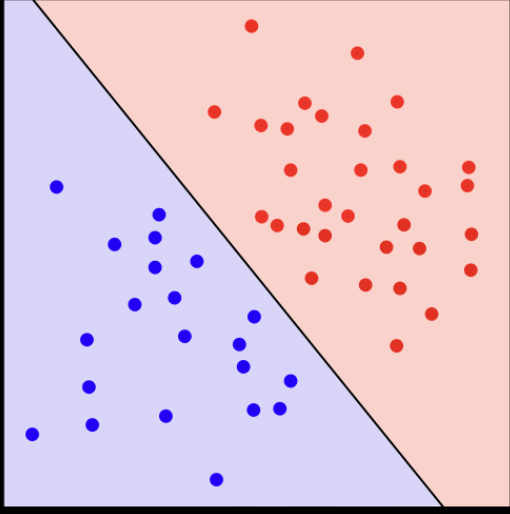
\includegraphics[width=\linewidth]{images/linearly_separable}
\end{figure}
\vspace{-0.6em}
{\tiny\centering \textbf{Linearly separable}: one straight line splits the two classes.\par}}
\end{column}
\end{columns}
\end{frame}


\begin{frame}

 \begin{mygreenbox}[title=Problem]
Prove that the following two sets are equal:
%
\begin{align*}
E &= \set{x \in \mathbb{Z}: x \text{\; is even}}, \text{and} \\
F &= \set{x \in \mathbb{Z}: x=a+b, \text{where $a$ and $b$ are both odd}}
\end{align*}
\end{mygreenbox}

\vfill 
 \begin{myyellowbox}[title=Puzzle]
Evaluate the proposed solution below (provided by a student last semester). 
\end{myyellowbox}

\vfill 
 \begin{myredbox}[title=Proposed Solution]
If $a$ and $b$ are both odd, then we can write $a=2c+1$ and $b=2d+1$, where both $c$ and $d$ are integers.  Now 
\[ a+b = (2c+1) + (2d+1) = 2c+2d+2 = 2(c+d+1).\]
That is, $a+b=2e$, where $e \defeq c+d+1$ is an integer.  Hence, $a+b$ is even.  Hence,  the sets $E$ and $F$ are equal. 
\end{myredbox}
\end{frame}


\begin{frame}{How to show two sets are equal}


 \begin{mygreenbox}[title=Proving two sets are equal]
To show $A=B$, we show $A \subseteq B$ and $B \subseteq A$.
\begin{itemize}
\item $\boxed{A \subseteq B.}$ We show that if $x \in A $, then $x \in B$.  
\item $\boxed{B \subseteq A.}$	We show that if $x \in B$, then $x \in A$.
\end{itemize}
\end{mygreenbox}	
\pause 
\begin{myredbox}[title=Visualization]

\begin{minipage}{0.48\textwidth}
\centering
\footnotesize The first bulletpoint shows
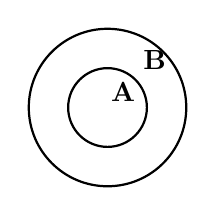
\begin{tikzpicture}
    % Draw Set B (larger set)
    \draw[thick] (0,0) circle (1.0cm);
    \node at (0.6,0.6) {\textbf{B}};

    % Draw Set A (nested inside B)
    \draw[thick] (0,0) circle (0.5cm);
    \node at (0.2,0.2) {\textbf{A}};
\end{tikzpicture}
\end{minipage}
\begin{minipage}{0.48\textwidth}
\centering
\footnotesize  The second bulletpoint shows
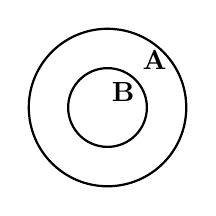
\begin{tikzpicture}
    % Draw Set B (larger set)
    \draw[thick] (0,0) circle (1.0cm);
    \node at (0.6,0.6) {\textbf{A}};

    % Draw Set A (nested inside B)
    \draw[thick] (0,0) circle (0.5cm);
    \node at (0.2,0.2) {\textbf{B}};
\end{tikzpicture}
\end{minipage}
\vfill
\centering 
Therefore
\vspace{0.1cm}
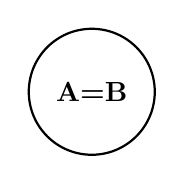
\begin{tikzpicture}
    % Draw Set B (larger set)
    \draw[thick] (0,0) circle (0.8cm);
    \node at (0.0,0.0) {\textbf{A=B}};
\end{tikzpicture}


\end{myredbox}

\end{frame}


\begin{frame}{How to show two sets are equal: Some intuition}
Suppose you're \alert{packing for a trip.} Your bag matches your checklist exactly when
\begin{enumerate}
	\item $\texttt{checklist} \subseteq \texttt{bag}$: nothing is \textbf{missing},
	\item $\texttt{bag} \subseteq \texttt{checklist}$: nothing \textbf{extra} snuck in.
\end{enumerate}

\vfill 

\begin{center}
   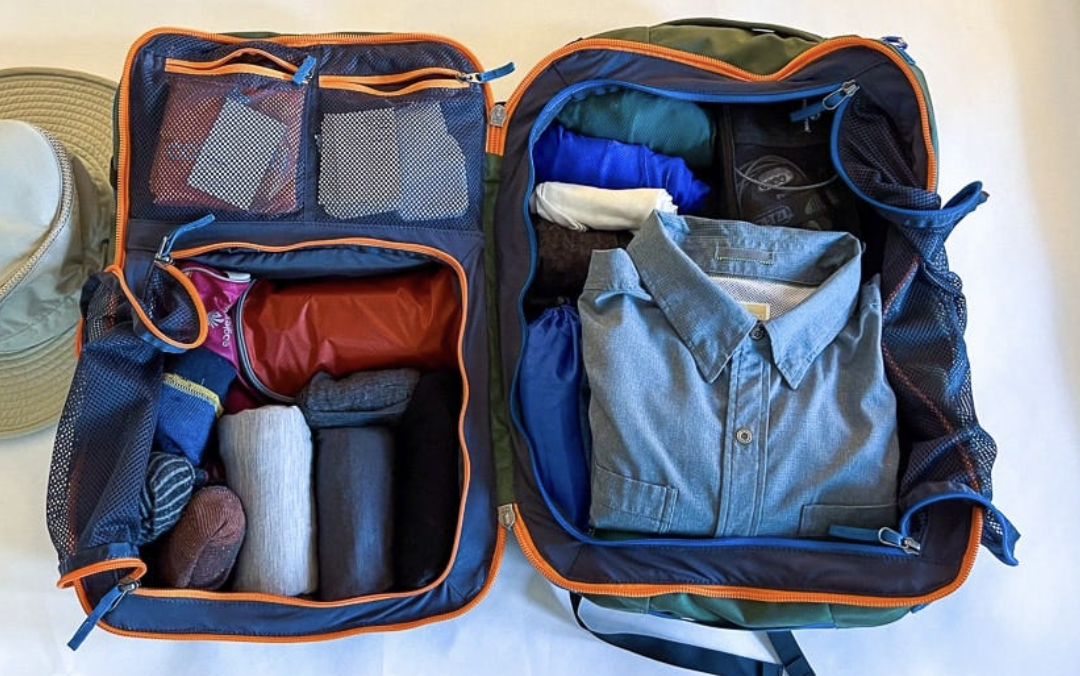
\includegraphics[width=.8\textwidth]{images/packing}   
\end{center}
\end{frame}



\begin{frame}{Solution to problem}
\small 

\textbf{Problem.} 
Prove that the following two sets are equal:
%
\begin{align*}
E &= \set{x \in \mathbb{Z}: x \text{\; is even}}, \text{and} \\
F &= \set{x \in \mathbb{Z}: x=a+b, \text{where $a$ and $b$ are both odd}}
\end{align*}


\vfill 
\textbf{Solution.} To show $E=F$, we show $E \subseteq F$ and $F \subseteq E$. \pause 
\begin{itemize}
\item $\boxed{F \subseteq E.}$	We show that if $x \in F$, then $x \in E$. Let $x \in F$.  \red{Hence $x=a+b$ for odd integers $a,b$.  By the definition of odd, we can write $a=(2c+1)$ and $b=(2d+1)$ for integers $c,d$.  Hence
\[x= a+b = (2c+1) + (2d+1) = 2c+2d+2 = 2 (c+d+1) \] 
That is, $a+b=2e$, where $e \defeq c+d+1$.  Hence, $a+b$ is even.} Hence, $x \in E$.
\pause 
\item $\boxed{E \subseteq F.}$ We show that if $x \in E $, then $x \in F$.  \pause Let $x \in E$.  Then $x=2a$ for some integer $a$.  Now we write	
\[ x=2a = \explaintermbrace{odd (by def.)}{(2a+1)} + \explaintermbrace{odd}{(-1)}\]  
Hence $x$ is the sum of two odd numbers.  Hence  $x \in F$.

\end{itemize}
\end{frame}







%%%% Section
\begin{frame}[standout]
Outline for Mini-Lecture:
\begin{itemize}
\item \textbullet \quad Introduction to sets and set notation
\item \textbullet \quad How to show two sets are equal
\item \alert{\textbullet \quad How to count the number of subsets}
\end{itemize}
\end{frame}



\begin{frame}{Counting Subsets}

\colorbox{yellow!30}{\textbf{Poll.}} Let $A=\set{a,b,c}$. How many subsets $S \subseteq A$ are there?

\vfill 
\pause 
\colorbox{green!30}{\textbf{Solution.}} There are $2 \times 2 \times 2 = 8$ subsets, because for each  element $x \in A$, we make a yes/no decision about whether to include $x$ in the subset. 

\vfill 
\pause 

\begin{figure}
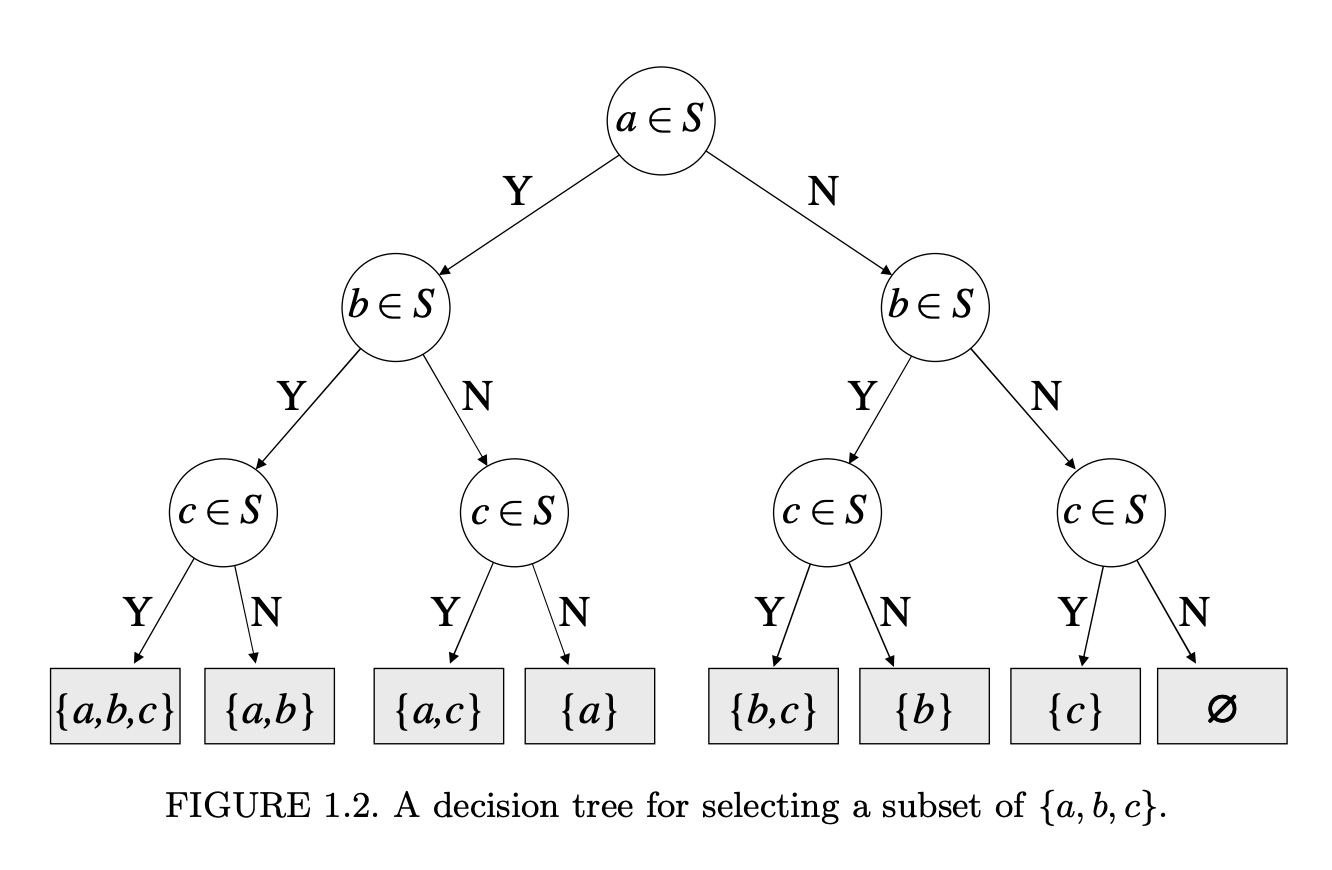
\includegraphics[width=.8\textwidth]{images/decision_tree}
%\tiny Source: Lovasz, Pelikan, Vesztergombi. \textit{Discrete Mathematics: Elementary and Beyond.} 	
\end{figure}

\end{frame}






\begin{frame}{Counting Subsets}
\small 
\colorbox{yellow!30}{\textbf{Poll.}} What does counting subsets have to do with lists?

\vfill 
\pause 

\colorbox{green!30}{\textbf{Explanation.}}  We can form a correspondence between lists and subsets since each subset is formed by a \texttt{yes} vs. \texttt{no} decision on whether to include each set item.  For example, if $A=\set{a,b,c}$, we have

\begin{center}
\begin{tabular}{rcl}
\textbf{List} & & \textbf{Subset} \\
(Y,Y,Y) & $\leftrightarrow$ &	$\set{a,b,c}$  \\
(Y,Y,N) & $\leftrightarrow$ &	 $\set{a,b}$  \\
(Y,N,Y) & $\leftrightarrow$ &	 $\set{a,c}$  \\
(Y,N,N) & $\leftrightarrow$ &	 $\set{a}$  \\
(N,Y,Y) & $\leftrightarrow$ &	 $\set{b,c}$  \\
(N,Y,N) & $\leftrightarrow$ &	 $\set{b}$  \\
(N,N,Y) & $\leftrightarrow$ &	 $\set{c}$  \\
(N,N,N) & $\leftrightarrow$ & 	$\emptyset$  \\
\end{tabular}
\end{center}
\vfill \pause 
Recall Scheinerman Theorem 8.6: \alert{the number of lists of length $k$ whose elements are chosen from a pool of $n$ elements is $n^k$ if repetitions are permitted.}  For counting subsets, $n=2$ (\texttt{yes} vs. \texttt{no}) and $k=|A|$.   In this case, we can form $2^{|A|} = 2^3 = 8$ such lists.

%\vfill 
%\pause 
%\begin{mygreenbox}[title= Reference: Theorem 8.6 from Scheinerman]
%The number of lists of length $k$ whose elements are chosen from a pool of $n$ elements 
%%
%\begin{align*}
%= \begin{cases}
% n^k, & \text{if repetitions are permitted} \\
% (n)_k, & \text{if repetitions are forbidden}	
% \end{cases}
%\end{align*}
%\end{mygreenbox}
 	
\end{frame}

\begin{frame}{Counting Subsets: Theorem}


Below we provide two versions of the same theorem.
\vfill 
\begin{mygreenbox}[title={Lovasz et al. Theorem 1.3.1}]
A set with $n$ elements has $2^n$ subsets.	
\end{mygreenbox}
\vfill 
\begin{myredbox}[title={Scheinerman Theorem 10.7}]
Let $A$ be a finite set.  The number of subsets of $A$ is $2^{|A|}$.	
\end{myredbox}

\end{frame}


\begin{frame}{Enumerating Subsets}

\begin{figure}
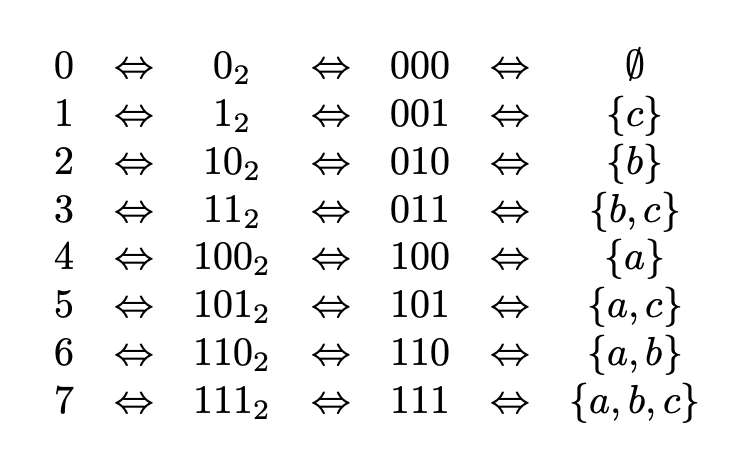
\includegraphics[width=.9\textwidth]{images/correspondence}

\tiny Source: Lovasz, Pelikan, Vesztergombi. \textit{Discrete Mathematics: Elementary and Beyond.} 	
\end{figure}

\vfill \vfill 
\footnotesize 
\textbf{Remark.} Using a code like this, you could determine that the 233rd subset of a 10-element set $\set{a_1, \hdots, a_{10}}$ consists of elements $\set{a_3, a_4, a_5, a_7, a_{10}}$. (That's because 233 in binary is 11101001, which corresponds to the code 0011101001.)
\end{frame}


\begin{frame}{Applications in computer science: Example}


\textbf{Feature selection in machine learning.} If you have $n$ possible features, there are $2^n$  possible subsets of features you could choose. Example: With 20 features, there are $2^{20} \approx$ 1 million possible subsets.

\end{frame}




\begin{frame}{Random group assignments}
\begin{columns}
\begin{column}{0.33\textwidth}
Ashley, Isabelle: 12 \\ 
Bailey, Tanna: 10 \\ 
Blaisdell, Olyver: 12 \\ 
Brown, Ashton: 13 \\ 
Brown, Jonathan: 1 \\ 
Cardenas, Dominic: 9 \\ 
Cutler, George: 13 \\ 
Fabik, Roland: 6 \\ 
Fellows, Audrey: 9 \\ 
Fitzgerald, Ryan: 7 \\ 
Fuller, Ryan: 11 \\ 
Griffen, Clara: 3 \\ 
Grutsch, Tanner: 4 \\\end{column}
\begin{column}{0.33\textwidth}
Hager, Nathan: 6 \\ 
Horner, Jayden: 10 \\ 
Johnson, Jaret: 7 \\ 
Kintzel, Samantha: 4 \\ 
Lameres, Alexis: 10 \\ 
Lee, Holden: 7 \\ 
Mayala, Reece: 8 \\ 
McLean, Connor: 2 \\ 
Mcbride, Daniel: 2 \\ 
Miller, Maverick: 11 \\ 
Moss, Emily: 9 \\ 
Mousseau, Matthew: 5 \\ 
Neuman, Evan: 8 \\\end{column}
\begin{column}{0.33\textwidth}
Putnam, John: 5 \\ 
Ramos, Vydel: 3 \\ 
Rathbun, Jedidiah: 8 \\ 
Roberts, Matthew: 11 \\ 
Roller, Nathan: 3 \\ 
Ryan, Otis: 2 \\ 
Shevtsov, Timothy: 5 \\ 
Sinclair, Aidan: 12 \\ 
Smith, Charles: 1 \\ 
Stensland, Emma: 1 \\ 
Thiessen, Logan: 6 \\ 
Thompson, Jaiden: 13 \\ 
Vath, Ethan: 4 \\\end{column}
\end{columns}

\end{frame}


\begin{frame}{Group exercises: Sets}


\begin{enumerate}
\item Find the cardinality of the following sets
\begin{itemize}
\item[a)] $\set{x \in \mathbb{Z}: |x| \leq 10}$
\item[b)] $\set{x \in \mathbb{Z}: 1 \leq x^2 \leq 2}$
\item[c)] $\set{x \in \mathbb{Z}: x \in \emptyset}$
\item[d)] $2^{2^{\set{1,2,3}}}$
\item[e)] $\set{x \in 2^{\set{1,2,3,4}}: |x|=1}$
\item[f)] $\set{\set{1,2}, \set{3,4,5}}$
\end{itemize}
\item Let $A= \set{x \in \mathbb{Z}: 4|x}$ and  $B= \set{x \in \mathbb{Z}: 2|x}$.  Prove that $A \subseteq B$.
\item Let $A= \set{0,1,2,3,4}$ and  $B= \set{x \in \mathbb{N}: x^2<17}$.  Prove that $A=B$.
\end{enumerate}

\end{frame}



\begin{frame}{Solution to group exercise \#1 (a-d)}

\small 
\textbf{Solution.}

\begin{itemize}
\item[a)] $\bigg|\set{x \in \mathbb{Z}: |x| \leq 10}\bigg|=\bigg| \set{-10, \hdots, -1, 0, 1, \hdots, 10} \bigg| = 21$ \pause 
\item[b)] $\bigg|\set{x \in \mathbb{Z}: 1 \leq x^2 \leq 2}\bigg| = \bigg| \set{-1, 1} \bigg| = 2 $ \pause 
\item[c)] $\bigg| \set{x \in \mathbb{Z}: x \in \emptyset} \bigg| = \bigg| \emptyset \bigg| = 0 $ \pause 
\item[d)] To find $\bigg|2^{2^{\set{1,2,3}}}\bigg|$, first recall from the text that for any finite set $A$, $2^A$ refers to the set of all subsets of $A$. So setting $A \defeq \set{1,2,3}$, we have 
\[ B \defeq 2^A = 2^{\set{1,2,3}} = \bigg\{ \emptyset, \set{1}, \set{2}, \set{3}, \set{1,2}, \set{1,3}, \set{2,3}, \set{1,2,3} \bigg\}. \]
Now  $2^B$ is the set of all subsets of \textit{that}, 
so
\[2^B = \bigg\{ \emptyset,  \big\{ \set{1}  \big\}, \big\{ \set{2} \big\}, \big\{  \set{3} \big\} , \big\{  \set{1},\set{2} \big\}, \hdots  \big\{  \set{1}, \set{1,2,3}, \set{2}, \set{1,2} \big\} , \hdots \bigg\}  \]
Notably, $B=2^A$ has $2^{|A|} = 2^3=8$ elements, and so $2^B$ has $2^{|B|} = 2^8$ elements. Hence,  $\bigg|2^{2^{\set{1,2,3}}}\bigg| = 2^8$. 
\end{itemize}


\end{frame}

\begin{frame}{Solution to group exercise \#1 (e-f)}

\small 
\textbf{Solution.}

\begin{itemize}
\item[e)] To find $\bigg| \set{x \in 2^{\set{1,2,3,4}}: |x|=1} \bigg|$, we proceed similarly as in part (d). The set  $B \defeq 2^{\set{1,2,3,4}}$ refers to the set of all subsets of $\set{1,2,3,4}$.  That is,  
\begin{align*}
 B &= \bigg\{ \emptyset, \set{1}, \set{2}, \set{3}, \set{4}, \set{1,2}, \set{1,3}, \set{1,4}, \set{2,4}, \hdots, \set{1,2,3,4} \bigg\}.	
\end{align*}

In particular $B$ has  $2^{|\set{1,2,3,4}|}=2^4=16$ elements.  Only four of those elements have cardinality 1, namely $\set{1}$, $\set{2}$, $\set{3}$, and $\set{4}$.  Hence $\bigg| \set{x \in 2^{\set{1,2,3,4}}: |x|=1} \bigg| = 4$. \pause 
\item[f)] $\bigg| \set{\set{1,2}, \set{3,4,5}} \bigg| = 2$
\end{itemize}


\end{frame}




\begin{frame}{Solution to group exercise \#2}


\textbf{Problem.} Let $A= \set{x \in \mathbb{Z}: 4|x}$ and  $B= \set{x \in \mathbb{Z}: 2|x}$.  Prove that $A \subseteq B$.
\vfill 
\textbf{Solution.} 

\begin{tabularx}{\textwidth}{|L{3cm}|X|}
\hline \textbf{Annotation} & \textbf{Main Text} \\ \hline
 \hlorange{Convert Prop. to ``if-then" form} &  \hlorange{We show that if $x \in A$, then $x \in B$.} \\ \hline
\hlblue{State assumption ("if")} & \hlblue{Let $x \in A$.} \\ \hline
\hlgreen{Unravel defs.} & \hlgreen{Since, $x\in A$, we know that $4|x$.  So by the definition of divisibility, there is some $n \in \mathbb{Z}$ such that $x=4n$.} \\ \hline
\hlred{*** The glue ***} & \hlred{We write $x=4n=2(2n)$} \\ \hline
 \hlgreen{Unravel defs.} & \hlgreen{So there is an integer $c=2n$ such that $x=2c$.  So $2|x$.} \\ \hline
  \hlblue{State conclusion} & \hlblue{Hence, $x \in B$.} \\ \hline
\hline
\end{tabularx}
\end{frame}



\begin{frame}{Solution to group exercise \#3 (Big picture)}


\textbf{Problem.} Let $A= \set{0,1,2,3,4}$ and  $B= \set{x \in \mathbb{N}: x^2<17}$.  Prove that $A=B$.

\vfill 
\textbf{Structure of solution.} To show $A=B$, we show $A \subseteq B$ and $B \subseteq A$.
\begin{itemize}
\item $\boxed{A \subseteq B.}$ We show that if $x \in A $, then $x \in B$.  
\item $\boxed{B \subseteq A.}$	We show that if $x \in B$, then $x \in A$.
\end{itemize}

\end{frame}


\begin{frame}{Solution to group exercise \#3}


\textbf{Problem.} Let $A= \set{0,1,2,3,4}$ and  $B= \set{x \in \mathbb{N}: x^2<17}$.  Prove that $A=B$.

\vfill 
\textbf{Solution.} To show $A=B$, we show $A \subseteq B$ and $B \subseteq A$. \pause 
\begin{itemize} 
\item $\boxed{A \subseteq B.}$ We show that if $x \in A $, then $x \in B$.  Let $x \in A$.  Then $x \in \set{0,1,2,3,4}$.  Then $x^2 \in \set{0,1,4,9,16}$.  So $x^2<17$.  Hence $x \in B$. \pause 
\item $\boxed{B \subseteq A.}$	We show that if $x \in B$, then $x \in A$. Let $x \in B$.  Hence $x \in \mathbb{N}$ and $x^2<17$.  By taking the square root of each side, $x^2<17$ implies   $|x|<\sqrt{17}$.   The only natural numbers satisfying $|x|<\sqrt{17}$ are $0,1,2,3$ and $4$.  Hence $x \in A$. 
\end{itemize}

\end{frame}


\end{document}
